\documentclass[12pt,a4paper]{article}
\usepackage[utf8]{inputenc}
\usepackage[english]{babel}
\usepackage{amsmath}
\usepackage{amsfonts}
\usepackage{amssymb}
\usepackage{makeidx}
\usepackage{graphicx}
\usepackage{kpfonts}
\usepackage{float}
\usepackage{multirow}
\usepackage{booktabs}
\usepackage[left=3cm,right=2cm,top=3cm,bottom=3cm]{geometry}
\author{Hélder Cruz}
\newcommand{\psil}{\psi_\text{l}}
\newcommand{\psill}{\psi_{\text{ll}}}
\newcommand{\psir}{\psi_\text{r}}
\newcommand{\psirr}{\psi_{\text{rr}}}
\begin{document}
In this tests we will consider this two attempts:
\begin{figure}[h]
\centering
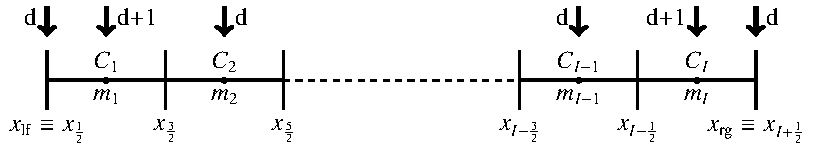
\includegraphics[width=\textwidth]{images/mesh_scheme_d_plus_1_old/mesh_scheme_d_plus_1_old}
\caption{Old attempt.}
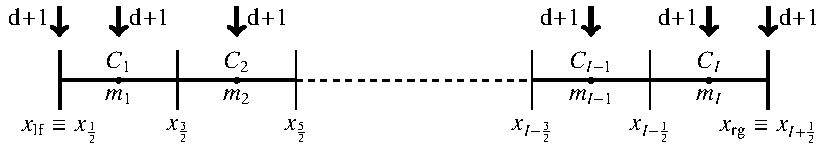
\includegraphics[width=\textwidth]{images/mesh_scheme_d_plus_1_new/mesh_scheme_d_plus_1_new}
\caption{New attempt.}
\end{figure}
\vspace{-0.5cm}
%=%=%=%=%=%=%=%=%=%=%=%=%=%=%=%=%=%=%=%=%=%=%=%=%=%=%=%=%=% 1
In this test we will consider:
\begin{itemize}
\item $\psi(x)=\exp(x)$
\item $\psil=1$;
\item $\psill=1$;
\item $\psir=1$;
\item $\psirr=1$;
\item $g(x)=-\exp(x)$.
\end{itemize}
\begin{table}[H]
\setlength{\tabcolsep}{5pt}
\centering
\caption{Test of 01\_01 with d and d+1 ($\exp(x)$ --- constant mesh).}
\resizebox{\linewidth}{!}{%
  \begin{tabular}{@{}l c c c c c c c c c c@{}}
\toprule
& & \multicolumn{4}{c}{$\omega=1|1$} &  & \multicolumn{4}{c}{$\omega=1|3$}\\
\cline{3-6} \cline{8-11} 
& $I$ & E$_{1}$ & $\mathcal O_{1}$ & E$_{\infty}$ & $\mathcal O_{\infty}$ &  & E$_{1}$ & $\mathcal O_{1}$ & E$_{\infty}$ & $\mathcal O_{\infty}$\\
\midrule
\multirow{4}{*}{$\mathbb{P}_{3}$}
 & 50 & 1.09E$-$05 & ---  & 1.72E$-$05 & --- &  & 8.41E$-$06 & --- & 1.36E$-$05 & ---\\
 & 100 & 1.34E$-$06 & 3.02  & 2.10E$-$06 & 3.03 &  & 1.02E$-$06 & 3.04 & 1.65E$-$06 & 3.04\\
 & 150 & 3.84E$-$07 & 3.08  & 5.99E$-$07 & 3.09 &  & 2.92E$-$07 & 3.10 & 4.68E$-$07 & 3.11\\
 & 200 & 1.57E$-$07 & 3.12  & 2.43E$-$07 & 3.14 &  & 1.17E$-$07 & 3.16 & 1.88E$-$07 & 3.16\\
\midrule
\multirow{4}{*}{$\mathbb{P}_{3}/\mathbb{P}_{4}$ (old)}
 & 50 & 2.46E$-$06 & ---  & 3.97E$-$06 & --- &  & 1.55E$-$06 & --- & 2.39E$-$06 & ---\\
 & 100 & 2.55E$-$07 & 3.27  & 4.01E$-$07 & 3.31 &  & 1.57E$-$07 & 3.31 & 2.20E$-$07 & 3.44\\
 & 150 & 6.01E$-$08 & 3.56  & 9.68E$-$08 & 3.51 &  & 3.33E$-$08 & 3.82 & 4.71E$-$08 & 3.80\\
 & 200 & 1.91E$-$08 & 3.99  & 3.38E$-$08 & 3.65 &  & 8.23E$-$09 & 4.86 & 1.53E$-$08 & 3.91\\
\midrule
\multirow{4}{*}{$\mathbb{P}_{3}/\mathbb{P}_{4}$ (new)}
 & 50 & 3.38E$-$06 & ---  & 6.75E$-$06 & --- &  & 1.31E$-$06 & --- & 2.11E$-$06 & ---\\
 & 100 & 6.77E$-$07 & 2.32  & 1.22E$-$06 & 2.47 &  & 1.43E$-$07 & 3.19 & 2.23E$-$07 & 3.24\\
 & 150 & 2.40E$-$07 & 2.56  & 4.14E$-$07 & 2.67 &  & 3.09E$-$08 & 3.77 & 5.31E$-$08 & 3.54\\
 & 200 & 1.10E$-$07 & 2.71  & 1.85E$-$07 & 2.79 &  & 7.66E$-$09 & 4.85 & 1.84E$-$08 & 3.69\\
\midrule
%
\multirow{4}{*}{$\mathbb{P}_{4}$}
 & 50 & 3.85E$-$07 & ---  & 7.68E$-$07 & --- &  & 3.08E$-$07 & --- & 6.06E$-$07 & ---\\
 & 100 & 1.11E$-$07 & 1.79  & 2.10E$-$07 & 1.87 &  & 9.29E$-$08 & 1.73 & 1.76E$-$07 & 1.78\\
 & 150 & 5.07E$-$08 & 1.93  & 9.53E$-$08 & 1.95 &  & 4.28E$-$08 & 1.91 & 8.06E$-$08 & 1.93\\
 & 200 & 2.88E$-$08 & 1.97  & 5.42E$-$08 & 1.96 &  & 2.44E$-$08 & 1.95 & 4.59E$-$08 & 1.95\\
\midrule
\multirow{4}{*}{$\mathbb{P}_{4}/\mathbb{P}_{5}$ (old)}
 & 50 & 4.20E$-$07 & ---  & 8.21E$-$07 & --- &  & 3.66E$-$07 & --- & 6.95E$-$07 & ---\\
 & 100 & 1.14E$-$07 & 1.88  & 2.14E$-$07 & 1.94 &  & 9.70E$-$08 & 1.92 & 1.82E$-$07 & 1.93\\
 & 150 & 5.10E$-$08 & 1.98  & 9.59E$-$08 & 1.99 &  & 4.36E$-$08 & 1.97 & 8.19E$-$08 & 1.98\\
 & 200 & 2.89E$-$08 & 1.97  & 5.44E$-$08 & 1.97 &  & 2.46E$-$08 & 2.00 & 4.61E$-$08 & 2.00\\
\midrule
\multirow{4}{*}{$\mathbb{P}_{4}/\mathbb{P}_{5}$ (new)}
 & 50 & 4.32E$-$07 & ---  & 8.31E$-$07 & --- &  & 3.75E$-$07 & --- & 7.09E$-$07 & ---\\
 & 100 & 1.14E$-$07 & 1.92  & 2.15E$-$07 & 1.95 &  & 9.76E$-$08 & 1.94 & 1.83E$-$07 & 1.95\\
 & 150 & 5.14E$-$08 & 1.97  & 9.64E$-$08 & 1.98 &  & 4.37E$-$08 & 1.98 & 8.21E$-$08 & 1.98\\
 & 200 & 2.90E$-$08 & 1.99  & 5.44E$-$08 & 1.99 &  & 2.46E$-$08 & 2.00 & 4.62E$-$08 & 2.00\\
\midrule
%
\multirow{4}{*}{$\mathbb{P}_{5}$}
 & 50 & 1.51E$-$09 & ---  & 2.16E$-$09 & --- &  & 9.32E$-$10 & --- & 1.46E$-$09 & ---\\
 & 100 & 3.51E$-$11 & 5.42  & 5.35E$-$11 & 5.34 &  & 2.82E$-$11 & 5.05 & 4.55E$-$11 & 5.00\\
 & 150 & 1.03E$-$12 & 8.69  & 2.29E$-$12 & 7.77 &  & 4.31E$-$12 & 4.64 & 8.16E$-$12 & 4.24\\
 & 200 & 7.66E$-$12 & $\uparrow$  & 1.72E$-$11 & $\uparrow$ &  & 1.27E$-$11 & $\uparrow$ & 2.52E$-$11 & $\uparrow$\\
\midrule
\multirow{4}{*}{$\mathbb{P}_{5}/\mathbb{P}_{6}$ (old)}
 & 50 & 7.22E$-$10 & ---  & 9.92E$-$10 & --- &  & 6.77E$-$10 & --- & 1.02E$-$09 & ---\\
 & 100 & 2.13E$-$11 & 5.09  & 3.29E$-$11 & 4.92 &  & 2.12E$-$11 & 4.99 & 3.32E$-$11 & 4.94\\
 & 150 & 1.51E$-$12 & 6.52  & 3.26E$-$12 & 5.70 &  & 5.91E$-$12 & 3.16 & 1.34E$-$11 & 2.24\\
 & 200 & 3.63E$-$12 & $\uparrow$  & 7.61E$-$12 & $\uparrow$ &  & 1.02E$-$11 & $\uparrow$ & 1.79E$-$11 & $\uparrow$\\
 \midrule
 \multirow{4}{*}{$\mathbb{P}_{5}/\mathbb{P}_{6}$ (new)}
 & 50 & 1.59E$-$09 & ---  & 2.43E$-$09 & --- &  & 5.19E$-$10 & --- & 8.43E$-$10 & ---\\
 & 100 & 2.91E$-$11 & 5.78  & 4.46E$-$11 & 5.77 &  & 1.53E$-$11 & 5.08 & 2.45E$-$11 & 5.10\\
 & 150 & 4.40E$-$12 & 4.66  & 7.42E$-$12 & 4.42 &  & 2.38E$-$12 & 4.59 & 5.77E$-$12 & 3.57\\
 & 200 & 6.46E$-$12 & $\uparrow$  & 1.27E$-$11 & $\uparrow$ &  & 6.74E$-$12 & $\uparrow$ & 1.58E$-$11 & $\uparrow$\\
\bottomrule
\end{tabular}}
\label{none}
\end{table}

\begin{table}[H]
\setlength{\tabcolsep}{5pt}
\centering
\caption{Test of 01\_01 with d and d+1 ($\exp(x)$ --- non-constant mesh).}
\resizebox{\linewidth}{!}{%
  \begin{tabular}{@{}l c c c c c c c c c c@{}}
\toprule
& & \multicolumn{4}{c}{$\omega=1|1$} &  & \multicolumn{4}{c}{$\omega=1|3$}\\
\cline{3-6} \cline{8-11} 
& $I$ & E$_{1}$ & $\mathcal O_{1}$ & E$_{\infty}$ & $\mathcal O_{\infty}$ &  & E$_{1}$ & $\mathcal O_{1}$ & E$_{\infty}$ & $\mathcal O_{\infty}$\\
\midrule
\multirow{4}{*}{$\mathbb{P}_{3}$}
 & 50 & 1.14E$-$05 & ---  & 1.79E$-$05 & --- &  & 7.04E$-$06 & --- & 1.05E$-$05 & ---\\
 & 100 & 1.30E$-$06 & 3.13  & 2.02E$-$06 & 3.15 &  & 6.72E$-$07 & 3.39 & 9.69E$-$07 & 3.44\\
 & 150 & 3.35E$-$07 & 3.35  & 5.18E$-$07 & 3.35 &  & 1.30E$-$07 & 4.05 & 2.12E$-$07 & 3.75\\
 & 200 & 1.18E$-$07 & 3.62  & 1.88E$-$07 & 3.53 &  & 2.65E$-$08 & 5.53 & 6.98E$-$08 & 3.85\\
\midrule
\multirow{4}{*}{$\mathbb{P}_{3}/\mathbb{P}_{4}$ (old)}
 & 50 & 1.95E$-$06 & ---  & 3.29E$-$06 & --- &  & 1.14E$-$06 & --- & 2.34E$-$06 & ---\\
 & 100 & 7.65E$-$08 & 4.67  & 2.33E$-$07 & 3.82 &  & 1.40E$-$07 & 3.03 & 3.01E$-$07 & 2.96\\
 & 150 & 5.94E$-$08 & 0.62  & 1.34E$-$07 & 1.37 &  & 1.03E$-$07 & 0.75 & 2.21E$-$07 & 0.76\\
 & 200 & 4.77E$-$08 & 0.77  & 1.03E$-$07 & 0.91 &  & 7.27E$-$08 & 1.22 & 1.50E$-$07 & 1.35\\
\midrule
\multirow{4}{*}{$\mathbb{P}_{3}/\mathbb{P}_{4}$ (new)}
 & 50 & 1.40E$-$06 & ---  & 2.30E$-$06 & --- &  & 3.20E$-$07 & --- & 8.76E$-$07 & ---\\
 & 100 & 2.42E$-$07 & 2.53  & 4.06E$-$07 & 2.50 &  & 2.10E$-$07 & 0.61 & 4.63E$-$07 & 0.92\\
 & 150 & 6.95E$-$08 & 3.08  & 1.36E$-$07 & 2.70 &  & 1.28E$-$07 & 1.22 & 2.66E$-$07 & 1.37\\
 & 200 & 2.25E$-$08 & 3.91  & 6.02E$-$08 & 2.83 &  & 8.32E$-$08 & 1.49 & 1.68E$-$07 & 1.60\\
\midrule
\multirow{4}{*}{$\mathbb{P}_{4}$}
 & 50 & 7.17E$-$08 & ---  & 1.61E$-$07 & --- &  & 7.74E$-$08 & --- & 1.31E$-$07 & ---\\
 & 100 & 3.09E$-$08 & 1.22  & 6.13E$-$08 & 1.39 &  & 2.80E$-$08 & 1.46 & 5.46E$-$08 & 1.26\\
 & 150 & 1.64E$-$08 & 1.55  & 3.16E$-$08 & 1.64 &  & 1.44E$-$08 & 1.65 & 2.75E$-$08 & 1.70\\
 & 200 & 1.01E$-$08 & 1.68  & 1.96E$-$08 & 1.66 &  & 8.52E$-$09 & 1.82 & 1.61E$-$08 & 1.84\\
\midrule
\multirow{4}{*}{$\mathbb{P}_{4}/\mathbb{P}_{5}$ (old)}
 & 50 & 1.50E$-$07 & ---  & 3.32E$-$07 & --- &  & 7.32E$-$08 & --- & 1.47E$-$07 & ---\\
 & 100 & 3.93E$-$08 & 1.94  & 7.45E$-$08 & 2.16 &  & 3.03E$-$08 & 1.27 & 5.84E$-$08 & 1.33\\
 & 150 & 1.69E$-$08 & 2.08  & 3.24E$-$08 & 2.05 &  & 1.49E$-$08 & 1.75 & 2.83E$-$08 & 1.78\\
 & 200 & 1.46E$-$08 & 0.51  & 2.67E$-$08 & 0.68 &  & 8.69E$-$09 & 1.87 & 1.64E$-$08 & 1.89\\
\midrule
\multirow{4}{*}{$\mathbb{P}_{4}/\mathbb{P}_{5}$ (new)}
 & 50 & 9.44E$-$08 & ---  & 2.11E$-$07 & --- &  & 1.04E$-$07 & --- & 2.05E$-$07 & ---\\
 & 100 & 3.74E$-$08 & 1.34  & 7.21E$-$08 & 1.55 &  & 3.29E$-$08 & 1.66 & 6.27E$-$08 & 1.71\\
 & 150 & 1.82E$-$08 & 1.77  & 3.44E$-$08 & 1.82 &  & 1.54E$-$08 & 1.87 & 2.92E$-$08 & 1.89\\
 & 200 & 1.02E$-$08 & 2.00  & 1.94E$-$08 & 1.98 &  & 8.86E$-$09 & 1.93 & 1.67E$-$08 & 1.94\\
\midrule
\multirow{4}{*}{$\mathbb{P}_{5}$}
 & 50 & 2.80E$-$09 & ---  & 4.63E$-$09 & --- &  & 2.25E$-$09 & --- & 3.76E$-$09 & ---\\
 & 100 & 1.17E$-$10 & 4.59  & 2.01E$-$10 & 4.53 &  & 1.07E$-$10 & 4.40 & 1.87E$-$10 & 4.33\\
 & 150 & 1.88E$-$11 & 4.50  & 3.31E$-$11 & 4.44 &  & 1.94E$-$11 & 4.20 & 3.49E$-$11 & 4.14\\
 & 200 & 4.60E$-$12 & 4.89  & 8.42E$-$12 & 4.76 &  & 7.54E$-$12 & 3.29 & 1.35E$-$11 & 3.29\\
\midrule
\multirow{4}{*}{$\mathbb{P}_{5}/\mathbb{P}_{6}$ (old)}
 & 50 & 2.33E$-$09 & ---  & 3.90E$-$09 & --- &  & 2.37E$-$09 & --- & 4.00E$-$09 & ---\\
 & 100 & 9.65E$-$11 & 4.59  & 1.68E$-$10 & 4.53 &  & 1.08E$-$10 & 4.46 & 1.89E$-$10 & 4.40\\
 & 150 & 1.44E$-$11 & 4.69  & 2.57E$-$11 & 4.64 &  & 1.74E$-$11 & 4.49 & 3.10E$-$11 & 4.47\\
 & 200 & 5.38E$-$12 & 3.42  & 9.70E$-$12 & 3.39 &  & 6.21E$-$12 & 3.58 & 1.08E$-$11 & 3.66\\
 \midrule
\multirow{4}{*}{$\mathbb{P}_{5}/\mathbb{P}_{6}$ (new)}
 & 50 & 5.59E$-$10 & ---  & 1.10E$-$09 & --- &  & 2.00E$-$10 & --- & 4.56E$-$10 & ---\\
 & 100 & 1.42E$-$11 & 5.30  & 2.71E$-$11 & 5.34 &  & 3.09E$-$11 & 2.69 & 6.53E$-$11 & 2.80\\
 & 150 & 5.27E$-$12 & 2.45  & 1.12E$-$11 & 2.17 &  & 9.05E$-$12 & 3.03 & 1.83E$-$11 & 3.13\\
 & 200 & 1.76E$-$12 & 3.82  & 3.66E$-$12 & 3.89 &  & 1.26E$-$11 & $\uparrow$ & 2.47E$-$11 & $\uparrow$\\
\bottomrule
\end{tabular}}
\label{none}
\end{table}

\pagebreak
%=%=%=%=%=%=%=%=%=%=%=%=%=%=%=%=%=%=%=%=%=%=%=%=%=%=%=%=%=% 2
In this test we will consider:
\begin{itemize}
\item $\psi(x)=-\exp(x)+\mathbb{P}_3$
\item $\psil=0$;
\item $\psill=0$;
\item $\psir=0$;
\item $\psirr=0$;
\item $g(x)=\exp(x)$.
\end{itemize}
\begin{table}[H]
\setlength{\tabcolsep}{5pt}
\centering
\caption{Test of 01\_01 with d and d+1 ($\exp(x)+\mathbb{P}_3$ --- constant mesh).}
\resizebox{\linewidth}{!}{%
  \begin{tabular}{@{}l c c c c c c c c c c@{}}
\toprule
& & \multicolumn{4}{c}{$\omega=1|1$} &  & \multicolumn{4}{c}{$\omega=1|3$}\\
\cline{3-6} \cline{8-11} 
& $I$ & E$_{1}$ & $\mathcal O_{1}$ & E$_{\infty}$ & $\mathcal O_{\infty}$ &  & E$_{1}$ & $\mathcal O_{1}$ & E$_{\infty}$ & $\mathcal O_{\infty}$\\
\midrule
\multirow{4}{*}{$\mathbb{P}_{3}$}
 & 50 & 1.09E$-$05 & ---  & 1.72E$-$05 & --- &  & 8.41E$-$06 & --- & 1.36E$-$05 & ---\\
 & 100 & 1.34E$-$06 & 3.02  & 2.10E$-$06 & 3.03 &  & 1.02E$-$06 & 3.04 & 1.65E$-$06 & 3.04\\
 & 150 & 3.84E$-$07 & 3.08  & 5.99E$-$07 & 3.09 &  & 2.92E$-$07 & 3.10 & 4.68E$-$07 & 3.11\\
 & 200 & 1.56E$-$07 & 3.12  & 2.43E$-$07 & 3.14 &  & 1.17E$-$07 & 3.16 & 1.88E$-$07 & 3.16\\
\midrule
\multirow{4}{*}{$\mathbb{P}_{3}/\mathbb{P}_{4}$ (old)}
 & 50 & 2.46E$-$06 & ---  & 3.97E$-$06 & --- &  & 1.55E$-$06 & --- & 2.39E$-$06 & ---\\
 & 100 & 2.55E$-$07 & 3.27  & 4.01E$-$07 & 3.31 &  & 1.57E$-$07 & 3.31 & 2.20E$-$07 & 3.44\\
 & 150 & 6.01E$-$08 & 3.56  & 9.68E$-$08 & 3.51 &  & 3.33E$-$08 & 3.82 & 4.71E$-$08 & 3.80\\
 & 200 & 1.91E$-$08 & 3.99  & 3.38E$-$08 & 3.65 &  & 8.32E$-$09 & 4.82 & 1.54E$-$08 & 3.88\\
\midrule
\multirow{4}{*}{$\mathbb{P}_{3}/\mathbb{P}_{4}$ (new)}
 & 50 & 3.38E$-$06 & ---  & 6.75E$-$06 & --- &  & 1.31E$-$06 & --- & 2.11E$-$06 & ---\\
 & 100 & 6.77E$-$07 & 2.32  & 1.22E$-$06 & 2.47 &  & 1.43E$-$07 & 3.19 & 2.23E$-$07 & 3.24\\
 & 150 & 2.40E$-$07 & 2.56  & 4.14E$-$07 & 2.67 &  & 3.09E$-$08 & 3.77 & 5.31E$-$08 & 3.54\\
 & 200 & 1.10E$-$07 & 2.71  & 1.85E$-$07 & 2.79 &  & 7.65E$-$09 & 4.86 & 1.84E$-$08 & 3.69\\
\midrule
\multirow{4}{*}{$\mathbb{P}_{4}$}
 & 50 & 3.85E$-$07 & ---  & 7.68E$-$07 & --- &  & 3.08E$-$07 & --- & 6.06E$-$07 & ---\\
 & 100 & 1.11E$-$07 & 1.79  & 2.10E$-$07 & 1.87 &  & 9.29E$-$08 & 1.73 & 1.76E$-$07 & 1.78\\
 & 150 & 5.07E$-$08 & 1.93  & 9.53E$-$08 & 1.95 &  & 4.28E$-$08 & 1.91 & 8.06E$-$08 & 1.93\\
 & 200 & 2.88E$-$08 & 1.97  & 5.41E$-$08 & 1.97 &  & 2.44E$-$08 & 1.96 & 4.58E$-$08 & 1.96\\
\midrule
\multirow{4}{*}{$\mathbb{P}_{4}/\mathbb{P}_{5}$ (old)}
 & 50 & 4.20E$-$07 & ---  & 8.21E$-$07 & --- &  & 3.66E$-$07 & --- & 6.95E$-$07 & ---\\
 & 100 & 1.14E$-$07 & 1.88  & 2.14E$-$07 & 1.94 &  & 9.70E$-$08 & 1.92 & 1.82E$-$07 & 1.93\\
 & 150 & 5.10E$-$08 & 1.98  & 9.59E$-$08 & 1.99 &  & 4.36E$-$08 & 1.97 & 8.19E$-$08 & 1.98\\
 & 200 & 2.89E$-$08 & 1.97  & 5.43E$-$08 & 1.98 &  & 2.46E$-$08 & 1.99 & 4.62E$-$08 & 1.99\\
\midrule
\multirow{4}{*}{$\mathbb{P}_{4}/\mathbb{P}_{5}$ (new)}
 & 50 & 4.32E$-$07 & ---  & 8.31E$-$07 & --- &  & 3.75E$-$07 & --- & 7.09E$-$07 & ---\\
 & 100 & 1.14E$-$07 & 1.92  & 2.15E$-$07 & 1.95 &  & 9.76E$-$08 & 1.94 & 1.83E$-$07 & 1.95\\
 & 150 & 5.14E$-$08 & 1.97  & 9.65E$-$08 & 1.98 &  & 4.37E$-$08 & 1.98 & 8.21E$-$08 & 1.98\\
 & 200 & 2.90E$-$08 & 1.99  & 5.44E$-$08 & 1.99 &  & 2.47E$-$08 & 1.99 & 4.63E$-$08 & 1.99\\
\midrule
\multirow{4}{*}{$\mathbb{P}_{5}$}
 & 50 & 1.51E$-$09 & ---  & 2.16E$-$09 & --- &  & 9.32E$-$10 & --- & 1.46E$-$09 & ---\\
 & 100 & 3.45E$-$11 & 5.45  & 5.37E$-$11 & 5.33 &  & 2.99E$-$11 & 4.96 & 4.79E$-$11 & 4.93\\
 & 150 & 4.20E$-$12 & 5.19  & 6.71E$-$12 & 5.13 &  & 3.72E$-$12 & 5.14 & 6.09E$-$12 & 5.09\\
 & 200 & 1.82E$-$12 & 2.92  & 2.88E$-$12 & 2.95 &  & 1.48E$-$12 & 3.21 & 2.38E$-$12 & 3.27\\
\midrule
\multirow{4}{*}{$\mathbb{P}_{5}/\mathbb{P}_{6}$ (old)}
 & 50 & 7.22E$-$10 & ---  & 9.93E$-$10 & --- &  & 6.77E$-$10 & --- & 1.02E$-$09 & ---\\
 & 100 & 2.40E$-$11 & 4.91  & 3.75E$-$11 & 4.73 &  & 2.18E$-$11 & 4.96 & 3.40E$-$11 & 4.90\\
 & 150 & 3.00E$-$12 & 5.13  & 4.82E$-$12 & 5.06 &  & 2.78E$-$12 & 5.09 & 4.44E$-$12 & 5.02\\
 & 200 & 1.23E$-$12 & 3.11  & 1.96E$-$12 & 3.13 &  & 1.09E$-$12 & 3.24 & 1.74E$-$12 & 3.25\\
\midrule
\multirow{4}{*}{$\mathbb{P}_{5}/\mathbb{P}_{6}$ (new)}
 & 50 & 1.59E$-$09 & ---  & 2.43E$-$09 & --- &  & 5.20E$-$10 & --- & 8.44E$-$10 & ---\\
 & 100 & 2.99E$-$11 & 5.74  & 4.61E$-$11 & 5.72 &  & 1.65E$-$11 & 4.97 & 2.60E$-$11 & 5.02\\
 & 150 & 1.92E$-$11 & 1.09  & 3.69E$-$11 & 0.55 &  & 2.03E$-$12 & 5.17 & 3.39E$-$12 & 5.03\\
 & 200 & 4.02E$-$11 & $\uparrow$  & 6.17E$-$11 & $\uparrow$ &  & 5.61E$-$13 & 4.47 & 9.74E$-$13 & 4.34\\
\bottomrule
\end{tabular}}
\label{none}
\end{table}

\begin{table}[H]
\setlength{\tabcolsep}{5pt}
\centering
\caption{Test of 01\_01 with d and d+1 ($\exp(x)+\mathbb{P}_3$ --- non-constant mesh).}
\resizebox{\linewidth}{!}{%
  \begin{tabular}{@{}l c c c c c c c c c c@{}}
\toprule
& & \multicolumn{4}{c}{$\omega=1|1$} &  & \multicolumn{4}{c}{$\omega=1|3$}\\
\cline{3-6} \cline{8-11} 
& $I$ & E$_{1}$ & $\mathcal O_{1}$ & E$_{\infty}$ & $\mathcal O_{\infty}$ &  & E$_{1}$ & $\mathcal O_{1}$ & E$_{\infty}$ & $\mathcal O_{\infty}$\\
\midrule
\multirow{4}{*}{$\mathbb{P}_{3}$}
 & 50 & 1.14E$-$05 & ---  & 1.79E$-$05 & --- &  & 7.04E$-$06 & --- & 1.05E$-$05 & ---\\
 & 100 & 1.30E$-$06 & 3.13  & 2.02E$-$06 & 3.15 &  & 6.72E$-$07 & 3.39 & 9.69E$-$07 & 3.44\\
 & 150 & 3.35E$-$07 & 3.35  & 5.18E$-$07 & 3.35 &  & 1.30E$-$07 & 4.05 & 2.12E$-$07 & 3.75\\
 & 200 & 1.18E$-$07 & 3.62  & 1.88E$-$07 & 3.53 &  & 2.65E$-$08 & 5.53 & 6.98E$-$08 & 3.85\\
\midrule
\multirow{4}{*}{$\mathbb{P}_{3}/\mathbb{P}_{4}$ (old)}
 & 50 & 1.95E$-$06 & ---  & 3.29E$-$06 & --- &  & 1.14E$-$06 & --- & 2.34E$-$06 & ---\\
 & 100 & 7.65E$-$08 & 4.67  & 2.33E$-$07 & 3.82 &  & 1.40E$-$07 & 3.03 & 3.01E$-$07 & 2.96\\
 & 150 & 5.94E$-$08 & 0.62  & 1.34E$-$07 & 1.37 &  & 1.03E$-$07 & 0.75 & 2.21E$-$07 & 0.76\\
 & 200 & 4.77E$-$08 & 0.77  & 1.03E$-$07 & 0.91 &  & 7.27E$-$08 & 1.22 & 1.50E$-$07 & 1.35\\
\midrule
\multirow{4}{*}{$\mathbb{P}_{3}/\mathbb{P}_{4}$ (new)}
 & 50 & 1.40E$-$06 & ---  & 2.30E$-$06 & --- &  & 3.20E$-$07 & --- & 8.76E$-$07 & ---\\
 & 100 & 2.42E$-$07 & 2.53  & 4.06E$-$07 & 2.50 &  & 2.10E$-$07 & 0.61 & 4.63E$-$07 & 0.92\\
 & 150 & 6.95E$-$08 & 3.08  & 1.36E$-$07 & 2.70 &  & 1.28E$-$07 & 1.22 & 2.66E$-$07 & 1.37\\
 & 200 & 2.25E$-$08 & 3.91  & 6.02E$-$08 & 2.83 &  & 8.32E$-$08 & 1.49 & 1.68E$-$07 & 1.60\\
\midrule
\multirow{4}{*}{$\mathbb{P}_{4}$}
 & 50 & 7.17E$-$08 & ---  & 1.61E$-$07 & --- &  & 7.74E$-$08 & --- & 1.31E$-$07 & ---\\
 & 100 & 3.09E$-$08 & 1.22  & 6.13E$-$08 & 1.39 &  & 2.80E$-$08 & 1.46 & 5.46E$-$08 & 1.26\\
 & 150 & 1.64E$-$08 & 1.55  & 3.16E$-$08 & 1.64 &  & 1.44E$-$08 & 1.65 & 2.75E$-$08 & 1.70\\
 & 200 & 1.01E$-$08 & 1.68  & 1.96E$-$08 & 1.66 &  & 8.52E$-$09 & 1.82 & 1.61E$-$08 & 1.85\\
\midrule
\multirow{4}{*}{$\mathbb{P}_{4}/\mathbb{P}_{5}$ (old)}
 & 50 & 1.50E$-$07 & ---  & 3.32E$-$07 & --- &  & 7.32E$-$08 & --- & 1.47E$-$07 & ---\\
 & 100 & 3.93E$-$08 & 1.94  & 7.45E$-$08 & 2.16 &  & 3.03E$-$08 & 1.27 & 5.84E$-$08 & 1.33\\
 & 150 & 1.69E$-$08 & 2.08  & 3.24E$-$08 & 2.05 &  & 1.49E$-$08 & 1.75 & 2.83E$-$08 & 1.78\\
 & 200 & 1.46E$-$08 & 0.51  & 2.67E$-$08 & 0.68 &  & 8.69E$-$09 & 1.87 & 1.64E$-$08 & 1.89\\
\midrule
\multirow{4}{*}{$\mathbb{P}_{4}/\mathbb{P}_{5}$ (new)}
 & 50 & 9.44E$-$08 & ---  & 2.11E$-$07 & --- &  & 1.04E$-$07 & --- & 2.05E$-$07 & ---\\
 & 100 & 3.74E$-$08 & 1.34  & 7.21E$-$08 & 1.55 &  & 3.29E$-$08 & 1.66 & 6.27E$-$08 & 1.71\\
 & 150 & 1.82E$-$08 & 1.77  & 3.44E$-$08 & 1.82 &  & 1.54E$-$08 & 1.87 & 2.92E$-$08 & 1.88\\
 & 200 & 1.02E$-$08 & 2.00  & 1.94E$-$08 & 1.98 &  & 8.86E$-$09 & 1.93 & 1.67E$-$08 & 1.94\\
\midrule
\multirow{4}{*}{$\mathbb{P}_{5}$}
 & 50 & 2.80E$-$09 & ---  & 4.63E$-$09 & --- &  & 2.25E$-$09 & --- & 3.76E$-$09 & ---\\
 & 100 & 1.17E$-$10 & 4.58  & 2.02E$-$10 & 4.52 &  & 1.07E$-$10 & 4.40 & 1.87E$-$10 & 4.33\\
 & 150 & 1.87E$-$11 & 4.53  & 3.28E$-$11 & 4.48 &  & 1.90E$-$11 & 4.25 & 3.39E$-$11 & 4.20\\
 & 200 & 6.09E$-$12 & 3.89  & 1.08E$-$11 & 3.85 &  & 4.71E$-$12 & 4.85 & 8.46E$-$12 & 4.83\\
\midrule
\multirow{4}{*}{$\mathbb{P}_{5}/\mathbb{P}_{6}$ (old)}
 & 50 & 2.33E$-$09 & ---  & 3.90E$-$09 & --- &  & 2.37E$-$09 & --- & 4.00E$-$09 & ---\\
 & 100 & 9.59E$-$11 & 4.60  & 1.67E$-$10 & 4.54 &  & 1.07E$-$10 & 4.47 & 1.89E$-$10 & 4.41\\
 & 150 & 1.61E$-$11 & 4.39  & 2.89E$-$11 & 4.33 &  & 1.84E$-$11 & 4.35 & 3.29E$-$11 & 4.31\\
 & 200 & 4.05E$-$12 & 4.81  & 7.24E$-$12 & 4.81 &  & 6.05E$-$12 & 3.86 & 1.10E$-$11 & 3.82\\
\midrule
\multirow{4}{*}{$\mathbb{P}_{5}/\mathbb{P}_{6}$ (new)}
 & 50 & 5.59E$-$10 & ---  & 1.10E$-$09 & --- &  & 2.00E$-$10 & --- & 4.56E$-$10 & ---\\
 & 100 & 1.37E$-$11 & 5.35  & 2.55E$-$11 & 5.43 &  & 3.11E$-$11 & 2.69 & 6.57E$-$11 & 2.79\\
 & 150 & 5.58E$-$12 & 2.21  & 1.19E$-$11 & 1.88 &  & 7.36E$-$12 & 3.55 & 1.50E$-$11 & 3.64\\
 & 200 & 1.15E$-$12 & 5.49  & 2.30E$-$12 & 5.71 &  & 6.08E$-$12 & 0.66 & 1.17E$-$11 & 0.86\\
\bottomrule
\end{tabular}}
\label{none}
\end{table}
\pagebreak
%=%=%=%=%=%=%=%=%=%=%=%=%=%=%=%=%=%=%=%=%=%=%=%=%=%=%=%=%=% 3
In this test we will consider:
\begin{itemize}
\item $\psi(x)=\sin(x)$
\item $\psil=0$;
\item $\psill=1$;
\item $\psir=\sin(1)$;
\item $\psirr=\cos(1)$;
\item $g(x)=-\sin(x)$.
\end{itemize}
\begin{table}[H]
\setlength{\tabcolsep}{5pt}
\centering
\caption{Test of 01\_01 with d and d+1 ($\sin(x)$ --- constant mesh).}
\resizebox{\linewidth}{!}{%
  \begin{tabular}{@{}l c c c c c c c c c c@{}}
\toprule
& & \multicolumn{4}{c}{$\omega=1|1$} &  & \multicolumn{4}{c}{$\omega=1|3$}\\
\cline{3-6} \cline{8-11} 
& $I$ & E$_{1}$ & $\mathcal O_{1}$ & E$_{\infty}$ & $\mathcal O_{\infty}$ &  & E$_{1}$ & $\mathcal O_{1}$ & E$_{\infty}$ & $\mathcal O_{\infty}$\\
\midrule
\multirow{4}{*}{$\mathbb{P}_{3}$}
 & 50 & 2.73E$-$06 & ---  & 4.84E$-$06 & --- &  & 2.30E$-$06 & --- & 4.05E$-$06 & ---\\
 & 100 & 3.57E$-$07 & 2.94  & 6.30E$-$07 & 2.94 &  & 3.03E$-$07 & 2.92 & 5.34E$-$07 & 2.92\\
 & 150 & 1.10E$-$07 & 2.91  & 1.93E$-$07 & 2.91 &  & 9.42E$-$08 & 2.89 & 1.65E$-$07 & 2.89\\
 & 200 & 4.80E$-$08 & 2.87  & 8.44E$-$08 & 2.88 &  & 4.15E$-$08 & 2.85 & 7.28E$-$08 & 2.86\\
\midrule
\multirow{4}{*}{$\mathbb{P}_{3}/\mathbb{P}_{4}$ (old)}
 & 50 & 7.68E$-$07 & ---  & 1.39E$-$06 & --- &  & 4.76E$-$07 & --- & 8.59E$-$07 & ---\\
 & 100 & 1.08E$-$07 & 2.83  & 1.91E$-$07 & 2.86 &  & 7.47E$-$08 & 2.67 & 1.33E$-$07 & 2.69\\
 & 150 & 3.57E$-$08 & 2.73  & 6.29E$-$08 & 2.74 &  & 2.63E$-$08 & 2.57 & 4.68E$-$08 & 2.57\\
 & 200 & 1.67E$-$08 & 2.64  & 2.94E$-$08 & 2.64 &  & 1.28E$-$08 & 2.50 & 2.29E$-$08 & 2.49\\
\midrule
\multirow{4}{*}{$\mathbb{P}_{3}/\mathbb{P}_{4}$ (new)}
 & 50 & 1.05E$-$06 & ---  & 2.41E$-$06 & --- &  & 4.78E$-$07 & --- & 8.80E$-$07 & ---\\
 & 100 & 2.09E$-$07 & 2.33  & 4.35E$-$07 & 2.47 &  & 7.92E$-$08 & 2.59 & 1.42E$-$07 & 2.63\\
 & 150 & 7.75E$-$08 & 2.44  & 1.53E$-$07 & 2.58 &  & 2.81E$-$08 & 2.55 & 5.01E$-$08 & 2.57\\
 & 200 & 3.76E$-$08 & 2.51  & 7.19E$-$08 & 2.62 &  & 1.37E$-$08 & 2.50 & 2.44E$-$08 & 2.50\\
\midrule
\multirow{4}{*}{$\mathbb{P}_{4}$}
 & 50 & 1.11E$-$07 & ---  & 2.30E$-$07 & --- &  & 1.03E$-$07 & --- & 2.05E$-$07 & ---\\
 & 100 & 3.12E$-$08 & 1.83  & 5.98E$-$08 & 1.94 &  & 2.71E$-$08 & 1.93 & 5.17E$-$08 & 1.99\\
 & 150 & 1.42E$-$08 & 1.94  & 2.70E$-$08 & 1.96 &  & 1.22E$-$08 & 1.97 & 2.31E$-$08 & 1.98\\
 & 200 & 8.08E$-$09 & 1.97  & 1.53E$-$08 & 1.97 &  & 6.92E$-$09 & 1.97 & 1.31E$-$08 & 1.98\\
\midrule
\multirow{4}{*}{$\mathbb{P}_{4}/\mathbb{P}_{5}$ (old)}
 & 50 & 1.19E$-$07 & ---  & 2.44E$-$07 & --- &  & 9.83E$-$08 & --- & 1.94E$-$07 & ---\\
 & 100 & 3.20E$-$08 & 1.90  & 6.09E$-$08 & 2.00 &  & 2.69E$-$08 & 1.87 & 5.13E$-$08 & 1.92\\
 & 150 & 1.43E$-$08 & 1.98  & 2.71E$-$08 & 1.99 &  & 1.22E$-$08 & 1.96 & 2.31E$-$08 & 1.97\\
 & 200 & 8.12E$-$09 & 1.97  & 1.54E$-$08 & 1.96 &  & 6.91E$-$09 & 1.97 & 1.31E$-$08 & 1.98\\
\midrule
\multirow{4}{*}{$\mathbb{P}_{4}/\mathbb{P}_{5}$ (new)}
 & 50 & 1.22E$-$07 & ---  & 2.40E$-$07 & --- &  & 1.03E$-$07 & --- & 2.00E$-$07 & ---\\
 & 100 & 3.21E$-$08 & 1.93  & 6.08E$-$08 & 1.98 &  & 2.73E$-$08 & 1.92 & 5.17E$-$08 & 1.95\\
 & 150 & 1.44E$-$08 & 1.97  & 2.73E$-$08 & 1.98 &  & 1.22E$-$08 & 1.97 & 2.31E$-$08 & 1.98\\
 & 200 & 8.14E$-$09 & 1.99  & 1.54E$-$08 & 1.99 &  & 6.86E$-$09 & 2.01 & 1.29E$-$08 & 2.02\\
\midrule
\multirow{4}{*}{$\mathbb{P}_{5}$}
 & 50 & 3.37E$-$10 & ---  & 5.16E$-$10 & --- &  & 2.20E$-$10 & --- & 3.75E$-$10 & ---\\
 & 100 & 6.59E$-$12 & 5.68  & 1.09E$-$11 & 5.56 &  & 6.92E$-$12 & 4.99 & 1.17E$-$11 & 5.01\\
 & 150 & 1.13E$-$12 & 4.35  & 1.90E$-$12 & 4.31 &  & 1.08E$-$12 & 4.59 & 1.90E$-$12 & 4.47\\
 & 200 & 6.04E$-$13 & 2.18  & 1.45E$-$12 & 0.94 &  & 4.82E$-$12 & $\uparrow$ & 1.18E$-$11 & $\uparrow$\\
\midrule
\multirow{4}{*}{$\mathbb{P}_{5}/\mathbb{P}_{6}$ (old)}
 & 50 & 1.49E$-$10 & ---  & 2.39E$-$10 & --- &  & 1.41E$-$10 & --- & 2.37E$-$10 & ---\\
 & 100 & 2.88E$-$12 & 5.69  & 5.23E$-$12 & 5.52 &  & 3.53E$-$12 & 5.32 & 6.26E$-$12 & 5.24\\
 & 150 & 4.39E$-$13 & 4.64  & 8.58E$-$13 & 4.46 &  & 1.17E$-$12 & 2.73 & 2.50E$-$12 & 2.27\\
 & 200 & 3.73E$-$13 & 0.57  & 5.76E$-$13 & 1.38 &  & 1.14E$-$12 & 0.09 & 2.11E$-$12 & 0.59\\
\midrule
\multirow{4}{*}{$\mathbb{P}_{5}/\mathbb{P}_{6}$ (new)}
 & 50 & 4.06E$-$10 & ---  & 6.44E$-$10 & --- &  & 1.46E$-$10 & --- & 2.60E$-$10 & ---\\
 & 100 & 8.36E$-$12 & 5.60  & 1.39E$-$11 & 5.53 &  & 5.27E$-$12 & 4.79 & 9.29E$-$12 & 4.81\\
 & 150 & 7.76E$-$13 & 5.86  & 1.23E$-$12 & 5.97 &  & 3.87E$-$13 & 6.44 & 7.53E$-$13 & 6.20\\
 & 200 & 2.47E$-$12 & $\uparrow$  & 4.43E$-$12 & $\uparrow$ &  & 5.13E$-$12 & $\uparrow$ & 9.48E$-$12 & $\uparrow$\\
\bottomrule
\end{tabular}}
\label{none}
\end{table}

\begin{table}[H]
\setlength{\tabcolsep}{5pt}
\centering
\caption{Test of 01\_01 with d and d+1 ($\sin(x)$ --- non-constant mesh).}
\resizebox{\linewidth}{!}{%
  \begin{tabular}{@{}l c c c c c c c c c c@{}}
\toprule
& & \multicolumn{4}{c}{$\omega=1|1$} &  & \multicolumn{4}{c}{$\omega=1|3$}\\
\cline{3-6} \cline{8-11} 
& $I$ & E$_{1}$ & $\mathcal O_{1}$ & E$_{\infty}$ & $\mathcal O_{\infty}$ &  & E$_{1}$ & $\mathcal O_{1}$ & E$_{\infty}$ & $\mathcal O_{\infty}$\\
\midrule
\multirow{4}{*}{$\mathbb{P}_{3}$}
 & 50 & 1.99E$-$06 & ---  & 3.18E$-$06 & --- &  & 1.66E$-$06 & --- & 2.69E$-$06 & ---\\
 & 100 & 2.87E$-$07 & 2.79  & 4.71E$-$07 & 2.75 &  & 2.57E$-$07 & 2.69 & 4.26E$-$07 & 2.66\\
 & 150 & 1.00E$-$07 & 2.59  & 1.68E$-$07 & 2.54 &  & 9.33E$-$08 & 2.50 & 1.58E$-$07 & 2.45\\
 & 200 & 4.93E$-$08 & 2.47  & 8.39E$-$08 & 2.41 &  & 4.69E$-$08 & 2.39 & 8.06E$-$08 & 2.34\\
\midrule
\multirow{4}{*}{$\mathbb{P}_{3}/\mathbb{P}_{4}$ (old)}
 & 50 & 8.43E$-$07 & ---  & 1.44E$-$06 & --- &  & 7.38E$-$07 & --- & 1.31E$-$06 & ---\\
 & 100 & 1.59E$-$07 & 2.41  & 2.82E$-$07 & 2.35 &  & 1.50E$-$07 & 2.30 & 2.73E$-$07 & 2.26\\
 & 150 & 6.44E$-$08 & 2.23  & 1.16E$-$07 & 2.19 &  & 6.26E$-$08 & 2.16 & 1.15E$-$07 & 2.13\\
 & 200 & 3.46E$-$08 & 2.16  & 6.30E$-$08 & 2.13 &  & 3.41E$-$08 & 2.11 & 6.32E$-$08 & 2.08\\
\midrule
\multirow{4}{*}{$\mathbb{P}_{3}/\mathbb{P}_{4}$ (new)}
 & 50 & 1.27E$-$06 & ---  & 2.25E$-$06 & --- &  & 7.26E$-$07 & --- & 1.28E$-$06 & ---\\
 & 100 & 2.46E$-$07 & 2.37  & 4.21E$-$07 & 2.42 &  & 1.53E$-$07 & 2.25 & 2.76E$-$07 & 2.22\\
 & 150 & 9.37E$-$08 & 2.38  & 1.61E$-$07 & 2.38 &  & 6.35E$-$08 & 2.16 & 1.16E$-$07 & 2.13\\
 & 200 & 4.78E$-$08 & 2.34  & 8.23E$-$08 & 2.32 &  & 3.45E$-$08 & 2.12 & 6.38E$-$08 & 2.09\\
\midrule
\multirow{4}{*}{$\mathbb{P}_{4}$}
 & 50 & 3.03E$-$07 & ---  & 6.50E$-$07 & --- &  & 2.79E$-$07 & --- & 5.61E$-$07 & ---\\
 & 100 & 1.08E$-$07 & 1.48  & 2.08E$-$07 & 1.65 &  & 9.37E$-$08 & 1.57 & 1.79E$-$07 & 1.65\\
 & 150 & 5.15E$-$08 & 1.83  & 9.74E$-$08 & 1.87 &  & 4.41E$-$08 & 1.86 & 8.33E$-$08 & 1.88\\
 & 200 & 2.99E$-$08 & 1.89  & 5.66E$-$08 & 1.88 &  & 2.54E$-$08 & 1.93 & 4.77E$-$08 & 1.94\\
\midrule
\multirow{4}{*}{$\mathbb{P}_{4}/\mathbb{P}_{5}$ (old)}
 & 50 & 4.29E$-$07 & ---  & 8.48E$-$07 & --- &  & 3.23E$-$07 & --- & 6.31E$-$07 & ---\\
 & 100 & 1.18E$-$07 & 1.86  & 2.22E$-$07 & 1.93 &  & 9.73E$-$08 & 1.73 & 1.84E$-$07 & 1.78\\
 & 150 & 5.22E$-$08 & 2.01  & 9.85E$-$08 & 2.01 &  & 4.49E$-$08 & 1.91 & 8.45E$-$08 & 1.92\\
 & 200 & 3.41E$-$08 & 1.47  & 6.30E$-$08 & 1.55 &  & 2.56E$-$08 & 1.95 & 4.81E$-$08 & 1.96\\
\midrule
\multirow{4}{*}{$\mathbb{P}_{4}/\mathbb{P}_{5}$ (new)}
 & 50 & 3.98E$-$07 & ---  & 7.89E$-$07 & --- &  & 3.65E$-$07 & --- & 7.00E$-$07 & ---\\
 & 100 & 1.16E$-$07 & 1.77  & 2.20E$-$07 & 1.84 &  & 1.00E$-$07 & 1.87 & 1.89E$-$07 & 1.89\\
 & 150 & 5.35E$-$08 & 1.92  & 1.01E$-$07 & 1.93 &  & 4.55E$-$08 & 1.95 & 8.55E$-$08 & 1.96\\
 & 200 & 3.02E$-$08 & 1.99  & 5.67E$-$08 & 1.99 &  & 2.58E$-$08 & 1.97 & 4.84E$-$08 & 1.98\\
\midrule
\multirow{4}{*}{$\mathbb{P}_{5}$}
 & 50 & 2.20E$-$10 & ---  & 3.18E$-$10 & --- &  & 1.69E$-$10 & --- & 2.60E$-$10 & ---\\
 & 100 & 3.96E$-$12 & 5.79  & 6.72E$-$12 & 5.57 &  & 4.98E$-$12 & 5.08 & 9.47E$-$12 & 4.78\\
 & 150 & 7.33E$-$13 & 4.16  & 1.72E$-$12 & 3.36 &  & 2.48E$-$12 & 1.72 & 4.76E$-$12 & 1.70\\
 & 200 & 5.79E$-$12 & $\uparrow$  & 1.10E$-$11 & $\uparrow$ &  & 5.93E$-$12 & $\uparrow$ & 1.29E$-$11 & $\uparrow$\\
\midrule
\multirow{4}{*}{$\mathbb{P}_{5}/\mathbb{P}_{6}$ (old)}
 & 50 & 1.55E$-$10 & ---  & 2.23E$-$10 & --- &  & 1.60E$-$10 & --- & 2.45E$-$10 & ---\\
 & 100 & 2.00E$-$12 & 6.28  & 4.15E$-$12 & 5.75 &  & 2.26E$-$12 & 6.15 & 4.67E$-$12 & 5.71\\
 & 150 & 3.96E$-$13 & 4.00  & 9.29E$-$13 & 3.69 &  & 5.67E$-$12 & $\uparrow$ & 1.13E$-$11 & $\uparrow$\\
 & 200 & 4.07E$-$12 & $\uparrow$  & 7.61E$-$12 & $\uparrow$ &  & 3.66E$-$12 & 1.52 & 7.71E$-$12 & 1.33\\
\midrule
\multirow{4}{*}{$\mathbb{P}_{5}/\mathbb{P}_{6}$ (new)}
 & 50 & 1.49E$-$10 & ---  & 2.48E$-$10 & --- &  & 7.00E$-$11 & --- & 1.35E$-$10 & ---\\
 & 100 & 3.89E$-$12 & 5.26  & 7.28E$-$12 & 5.09 &  & 1.40E$-$12 & 5.65 & 3.62E$-$12 & 5.22\\
 & 150 & 1.78E$-$12 & 1.93  & 3.17E$-$12 & 2.05 &  & 2.82E$-$12 & $\uparrow$ & 5.65E$-$12 & $\uparrow$\\
 & 200 & 4.48E$-$12 & $\uparrow$  & 8.97E$-$12 & $\uparrow$ &  & 1.37E$-$11 & $\uparrow$ & 2.69E$-$11 & $\uparrow$\\
\bottomrule
\end{tabular}}
\label{none}
\end{table}
\pagebreak
%=%=%=%=%=%=%=%=%=%=%=%=%=%=%=%=%=%=%=%=%=%=%=%=%=%=%=%=%=% 4
In this test we will consider:
\begin{itemize}
\item $\psi(x)=x^4$
\item $\psil=0$;
\item $\psill=0$;
\item $\psir=1$;
\item $\psirr=4$;
\item $g(x)=-24$.
\end{itemize}
\begin{table}[H]
\setlength{\tabcolsep}{5pt}
\centering
\caption{Test of 01\_01 with d and d+1 ($x^4$ --- constant mesh).}
\resizebox{\linewidth}{!}{%
  \begin{tabular}{@{}l c c c c c c c c c c@{}}
\toprule
& & \multicolumn{4}{c}{$\omega=1|1$} &  & \multicolumn{4}{c}{$\omega=1|3$}\\
\cline{3-6} \cline{8-11} 
& $I$ & E$_{1}$ & $\mathcal O_{1}$ & E$_{\infty}$ & $\mathcal O_{\infty}$ &  & E$_{1}$ & $\mathcal O_{1}$ & E$_{\infty}$ & $\mathcal O_{\infty}$\\
\midrule
\multirow{4}{*}{$\mathbb{P}_{3}$}
 & 50 & 1.47E$-$04 & ---  & 2.22E$-$04 & --- &  & 1.08E$-$04 & --- & 1.65E$-$04 & ---\\
 & 100 & 1.86E$-$05 & 2.98  & 2.80E$-$05 & 2.99 &  & 1.36E$-$05 & 2.98 & 2.07E$-$05 & 2.99\\
 & 150 & 5.54E$-$06 & 2.99  & 8.33E$-$06 & 2.99 &  & 4.08E$-$06 & 2.98 & 6.18E$-$06 & 2.98\\
 & 200 & 2.34E$-$06 & 3.00  & 3.51E$-$06 & 3.00 &  & 1.76E$-$06 & 2.92 & 2.67E$-$06 & 2.92\\
\midrule
\multirow{4}{*}{$\mathbb{P}_{3}/\mathbb{P}_{4}$ (old)}
 & 50 & 3.71E$-$05 & ---  & 5.71E$-$05 & --- &  & 2.92E$-$05 & --- & 4.67E$-$05 & ---\\
 & 100 & 4.56E$-$06 & 3.02  & 6.92E$-$06 & 3.04 &  & 3.81E$-$06 & 2.94 & 5.97E$-$06 & 2.97\\
 & 150 & 1.34E$-$06 & 3.02  & 2.03E$-$06 & 3.02 &  & 1.17E$-$06 & 2.92 & 1.81E$-$06 & 2.94\\
 & 200 & 6.18E$-$07 & 2.70  & 9.33E$-$07 & 2.70 &  & 5.31E$-$07 & 2.74 & 8.15E$-$07 & 2.78\\
\midrule
\multirow{4}{*}{$\mathbb{P}_{3}/\mathbb{P}_{4}$ (new)}
 & 50 & 4.90E$-$05 & ---  & 8.07E$-$05 & --- &  & 2.34E$-$05 & --- & 3.71E$-$05 & ---\\
 & 100 & 1.01E$-$05 & 2.28  & 1.59E$-$05 & 2.34 &  & 3.28E$-$06 & 2.84 & 5.05E$-$06 & 2.87\\
 & 150 & 3.68E$-$06 & 2.49  & 5.72E$-$06 & 2.53 &  & 9.59E$-$07 & 3.03 & 1.65E$-$06 & 2.76\\
 & 200 & 4.15E$-$06 & $\uparrow$  & 8.40E$-$06 & $\uparrow$ &  & 3.98E$-$07 & 3.05 & 7.35E$-$07 & 2.81\\
\midrule
\multirow{4}{*}{$\mathbb{P}_{4}$}
 & 50 & 3.39E$-$12 & ---  & 6.47E$-$12 & --- &  & 2.38E$-$12 & --- & 4.74E$-$12 & ---\\
 & 100 & 7.61E$-$11 & $\uparrow$  & 1.36E$-$10 & $\uparrow$ &  & 2.51E$-$11 & $\uparrow$ & 4.14E$-$11 & $\uparrow$\\
 & 150 & 8.79E$-$11 & $\uparrow$  & 1.71E$-$10 & $\uparrow$ &  & 2.17E$-$11 & 0.36 & 4.09E$-$11 & 0.03\\
 & 200 & 2.94E$-$10 & $\uparrow$  & 5.78E$-$10 & $\uparrow$ &  & 7.77E$-$11 & $\uparrow$ & 1.15E$-$10 & $\uparrow$\\
\midrule
\multirow{4}{*}{$\mathbb{P}_{4}/\mathbb{P}_{5}$ (old)}
 & 50 & 4.97E$-$11 & ---  & 9.61E$-$11 & --- &  & 2.76E$-$11 & --- & 5.33E$-$11 & ---\\
 & 100 & 7.28E$-$12 & 2.77  & 1.20E$-$11 & 3.00 &  & 4.54E$-$12 & 2.60 & 7.62E$-$12 & 2.80\\
 & 150 & 1.95E$-$11 & $\uparrow$  & 2.99E$-$11 & $\uparrow$ &  & 3.68E$-$12 & 0.52 & 5.93E$-$12 & 0.62\\
 & 200 & 1.00E$-$11 & 2.31  & 2.02E$-$11 & 1.36 &  & 1.14E$-$11 & $\uparrow$ & 2.31E$-$11 & $\uparrow$\\
\midrule
\multirow{4}{*}{$\mathbb{P}_{4}/\mathbb{P}_{5}$ (new)}
 & 50 & 1.83E$-$14 & ---  & 4.88E$-$14 & --- &  & 6.14E$-$11 & --- & 1.06E$-$10 & ---\\
 & 100 & 8.31E$-$09 & $\uparrow$  & 1.72E$-$08 & $\uparrow$ &  & 1.66E$-$10 & $\uparrow$ & 2.51E$-$10 & $\uparrow$\\
 & 150 & 2.48E$-$08 & $\uparrow$  & 4.61E$-$08 & $\uparrow$ &  & 1.28E$-$09 & $\uparrow$ & 2.28E$-$09 & $\uparrow$\\
 & 200 & 1.18E$-$07 & $\uparrow$  & 3.16E$-$07 & $\uparrow$ &  & 7.23E$-$10 & 1.98 & 1.52E$-$09 & 1.40\\
\midrule
\multirow{4}{*}{$\mathbb{P}_{5}$}
 & 50 & 1.82E$-$12 & ---  & 3.63E$-$12 & --- &  & 1.78E$-$12 & --- & 3.20E$-$12 & ---\\
 & 100 & 4.34E$-$11 & $\uparrow$  & 8.40E$-$11 & $\uparrow$ &  & 3.49E$-$11 & $\uparrow$ & 7.02E$-$11 & $\uparrow$\\
 & 150 & 1.51E$-$09 & $\uparrow$  & 2.28E$-$09 & $\uparrow$ &  & 9.52E$-$10 & $\uparrow$ & 1.46E$-$09 & $\uparrow$\\
 & 200 & 1.56E$-$09 & $\uparrow$  & 2.52E$-$09 & $\uparrow$ &  & 1.13E$-$09 & $\uparrow$ & 1.82E$-$09 & $\uparrow$\\
\midrule
\multirow{4}{*}{$\mathbb{P}_{5}/\mathbb{P}_{6}$ (old)}
 & 50 & 1.56E$-$12 & ---  & 2.46E$-$12 & --- &  & 1.41E$-$12 & --- & 2.20E$-$12 & ---\\
 & 100 & 2.72E$-$11 & $\uparrow$  & 5.42E$-$11 & $\uparrow$ &  & 1.96E$-$11 & $\uparrow$ & 3.92E$-$11 & $\uparrow$\\
 & 150 & 9.62E$-$10 & $\uparrow$  & 1.44E$-$09 & $\uparrow$ &  & 7.51E$-$10 & $\uparrow$ & 1.14E$-$09 & $\uparrow$\\
 & 200 & 1.02E$-$09 & $\uparrow$  & 1.64E$-$09 & $\uparrow$ &  & 8.48E$-$10 & $\uparrow$ & 1.40E$-$09 & $\uparrow$\\
\midrule
\multirow{4}{*}{$\mathbb{P}_{5}/\mathbb{P}_{6}$}
 & 50 & 1.96E$-$09 & ---  & 2.89E$-$09 & --- &  & 3.52E$-$11 & --- & 6.05E$-$11 & ---\\
 & 100 & 1.41E$-$07 & $\uparrow$  & 2.10E$-$07 & $\uparrow$ &  & 1.47E$-$09 & $\uparrow$ & 2.92E$-$09 & $\uparrow$\\
 & 150 & 1.43E$-$07 & $\uparrow$  & 2.30E$-$07 & $\uparrow$ &  & 3.23E$-$09 & $\uparrow$ & 5.71E$-$09 & $\uparrow$\\
 & 200 & 1.80E$-$06 & $\uparrow$  & 2.86E$-$06 & $\uparrow$ &  & 3.21E$-$09 & 0.02 & 5.71E$-$09 & $\uparrow$\\ 
\bottomrule
\end{tabular}}
\label{none}
\end{table}

\begin{table}[H]
\setlength{\tabcolsep}{5pt}
\centering
\caption{Test of 01\_01 with d and d+1 ($x^4$ --- non-constant mesh).}
\resizebox{\linewidth}{!}{%
  \begin{tabular}{@{}l c c c c c c c c c c@{}}
\toprule
& & \multicolumn{4}{c}{$\omega=1|1$} &  & \multicolumn{4}{c}{$\omega=1|3$}\\
\cline{3-6} \cline{8-11} 
& $I$ & E$_{1}$ & $\mathcal O_{1}$ & E$_{\infty}$ & $\mathcal O_{\infty}$ &  & E$_{1}$ & $\mathcal O_{1}$ & E$_{\infty}$ & $\mathcal O_{\infty}$\\
\midrule
\multirow{4}{*}{$\mathbb{P}_{3}$}
 & 50 & 1.96E$-$04 & ---  & 3.38E$-$04 & --- &  & 1.02E$-$04 & --- & 1.73E$-$04 & ---\\
 & 100 & 2.03E$-$05 & 3.27  & 3.66E$-$05 & 3.20 &  & 5.90E$-$06 & 4.11 & 1.52E$-$05 & 3.51\\
 & 150 & 4.32E$-$06 & 3.82  & 9.03E$-$06 & 3.45 &  & 1.85E$-$06 & 2.86 & 3.41E$-$06 & 3.69\\
 & 200 & 1.08E$-$06 & 4.83  & 3.20E$-$06 & 3.61 &  & 1.50E$-$06 & 0.73 & 3.21E$-$06 & 0.21\\
\midrule
\multirow{4}{*}{$\mathbb{P}_{3}/\mathbb{P}_{4}$ (old)}
 & 50 & 1.74E$-$05 & ---  & 5.22E$-$05 & --- &  & 1.38E$-$05 & --- & 3.48E$-$05 & ---\\
 & 100 & 5.05E$-$06 & 1.79  & 1.11E$-$05 & 2.23 &  & 7.80E$-$06 & 0.82 & 1.65E$-$05 & 1.08\\
 & 150 & 3.31E$-$06 & 1.04  & 6.89E$-$06 & 1.17 &  & 4.55E$-$06 & 1.33 & 9.22E$-$06 & 1.44\\
 & 200 & 2.20E$-$06 & 1.42  & 4.44E$-$06 & 1.53 &  & 2.90E$-$06 & 1.57 & 5.74E$-$06 & 1.65\\
\midrule
\multirow{4}{*}{$\mathbb{P}_{3}/\mathbb{P}_{4}$ (new)}
 & 50 & 2.59E$-$05 & ---  & 5.48E$-$05 & --- &  & 2.66E$-$05 & --- & 5.84E$-$05 & ---\\
 & 100 & 5.02E$-$06 & 2.37  & 1.06E$-$05 & 2.37 &  & 1.02E$-$05 & 1.38 & 2.07E$-$05 & 1.50\\
 & 150 & 2.28E$-$06 & 1.95  & 4.82E$-$06 & 1.95 &  & 5.26E$-$06 & 1.64 & 1.04E$-$05 & 1.71\\
 & 200 & 1.38E$-$06 & 1.74  & 2.93E$-$06 & 1.74 &  & 3.19E$-$06 & 1.74 & 6.21E$-$06 & 1.79\\
\midrule
\multirow{4}{*}{$\mathbb{P}_{4}$}
 & 50 & 9.79E$-$14 & ---  & 1.86E$-$13 & --- &  & 3.31E$-$13 & --- & 6.33E$-$13 & ---\\
 & 100 & 2.92E$-$13 & $\uparrow$  & 5.95E$-$13 & $\uparrow$ &  & 1.49E$-$12 & $\uparrow$ & 2.86E$-$12 & $\uparrow$\\
 & 150 & 6.92E$-$13 & $\uparrow$  & 1.74E$-$12 & $\uparrow$ &  & 6.43E$-$12 & $\uparrow$ & 1.28E$-$11 & $\uparrow$\\
 & 200 & 2.41E$-$12 & $\uparrow$  & 5.94E$-$12 & $\uparrow$ &  & 1.15E$-$11 & $\uparrow$ & 2.73E$-$11 & $\uparrow$\\
\midrule
\multirow{4}{*}{$\mathbb{P}_{4}/\mathbb{P}_{5}$ (old)}
 & 50 & 5.64E$-$14 & ---  & 1.23E$-$13 & --- &  & 6.20E$-$14 & --- & 1.15E$-$13 & ---\\
 & 100 & 6.94E$-$13 & $\uparrow$  & 1.34E$-$12 & $\uparrow$ &  & 2.13E$-$12 & $\uparrow$ & 4.26E$-$12 & $\uparrow$\\
 & 150 & 1.60E$-$12 & $\uparrow$  & 3.41E$-$12 & $\uparrow$ &  & 5.21E$-$12 & $\uparrow$ & 1.12E$-$11 & $\uparrow$\\
 & 200 & 2.39E$-$12 & $\uparrow$  & 4.90E$-$12 & $\uparrow$ &  & 2.72E$-$11 & $\uparrow$ & 5.53E$-$11 & $\uparrow$\\
\midrule
\multirow{4}{*}{$\mathbb{P}_{4}/\mathbb{P}_{5}$ (new)}
 & 50 & 2.23E$-$13 & ---  & 4.42E$-$13 & --- &  & 5.35E$-$13 & --- & 1.01E$-$12 & ---\\
 & 100 & 2.84E$-$13 & $\uparrow$  & 5.32E$-$13 & $\uparrow$ &  & 9.65E$-$13 & $\uparrow$ & 2.16E$-$12 & $\uparrow$\\
 & 150 & 2.74E$-$12 & $\uparrow$  & 5.22E$-$12 & $\uparrow$ &  & 1.58E$-$12 & $\uparrow$ & 3.40E$-$12 & $\uparrow$\\
 & 200 & 2.92E$-$12 & $\uparrow$  & 6.70E$-$12 & $\uparrow$ &  & 3.81E$-$11 & $\uparrow$ & 7.19E$-$11 & $\uparrow$\\
\midrule
\multirow{4}{*}{$\mathbb{P}_{5}$}
 & 50 & 9.79E$-$14 & ---  & 1.57E$-$13 & --- &  & 2.35E$-$13 & --- & 4.91E$-$13 & ---\\
 & 100 & 2.09E$-$12 & $\uparrow$  & 4.13E$-$12 & $\uparrow$ &  & 4.17E$-$12 & $\uparrow$ & 8.43E$-$12 & $\uparrow$\\
 & 150 & 2.94E$-$12 & $\uparrow$  & 5.22E$-$12 & $\uparrow$ &  & 6.53E$-$12 & $\uparrow$ & 1.34E$-$11 & $\uparrow$\\
 & 200 & 1.15E$-$11 & $\uparrow$  & 2.48E$-$11 & $\uparrow$ &  & 2.09E$-$11 & $\uparrow$ & 4.12E$-$11 & $\uparrow$\\
\midrule
\multirow{4}{*}{$\mathbb{P}_{5}/\mathbb{P}_{6}$ (old)}
 & 50 & 9.42E$-$14 & ---  & 1.69E$-$13 & --- &  & 6.24E$-$13 & --- & 1.21E$-$12 & ---\\
 & 100 & 2.25E$-$12 & $\uparrow$  & 4.30E$-$12 & $\uparrow$ &  & 3.95E$-$12 & $\uparrow$ & 7.44E$-$12 & $\uparrow$\\
 & 150 & 5.83E$-$13 & 3.33  & 1.60E$-$12 & 2.44 &  & 1.37E$-$11 & $\uparrow$ & 2.71E$-$11 & $\uparrow$\\
 & 200 & 2.71E$-$12 & $\uparrow$  & 6.11E$-$12 & $\uparrow$ &  & 1.97E$-$11 & $\uparrow$ & 4.26E$-$11 & $\uparrow$\\
\midrule
\multirow{4}{*}{$\mathbb{P}_{5}/\mathbb{P}_{6}$ (new)}
 & 50 & 2.46E$-$13 & ---  & 4.75E$-$13 & --- &  & 1.79E$-$13 & --- & 3.42E$-$13 & ---\\
 & 100 & 2.47E$-$12 & $\uparrow$  & 4.67E$-$12 & $\uparrow$ &  & 2.24E$-$12 & $\uparrow$ & 4.56E$-$12 & $\uparrow$\\
 & 150 & 4.09E$-$13 & 4.44  & 8.24E$-$13 & 4.28 &  & 9.28E$-$12 & $\uparrow$ & 1.83E$-$11 & $\uparrow$\\
 & 200 & 6.53E$-$12 & $\uparrow$  & 1.52E$-$11 & $\uparrow$ &  & 3.62E$-$11 & $\uparrow$ & 6.77E$-$11 & $\uparrow$\\
\bottomrule
\end{tabular}}
\label{none}
\end{table}

\end{document}